% Inhalte des Papers (grob), Schwerpunkte (Verbesserungen in Tor gegenüber damals existierenden Systemen), Neuerungen in Tor, etc.
%Mal schauen, eher beide...

%-Verbeserungen zu Onion routing:
%aus dem abstract: 
%by adding perfect forward secrecy, 
%congestion control, 
%directory servers,
%integrity checking, 
%configurable exit policies, 
%and a practical design for location-hidden services via rendezvous points.


% How does Tor work? Onion proxy, onion router, TLS link encryption, cells, constructing a circuit, sending data (HTTP, ...)
% Chapter6: Other design decisions: DoS, Exit policies and abuse, dirrectory servers



\section{Tor}

The details mentioned in this section are taken from \cite{tor2004original} if not stated otherwise.

Tor is a circuit-based low-latency service providing anonymous communication improving the concepts of the already explained onion routing. It is designed to anonymize TCP connections. This enables Tor to work with most standard applications of the net like HTTP to visit websites and other application layer protocols.

Users of the network use an \textbf{onion proxy} to connect their TCP connections to the Tor network. They establish a circuit through the network containing several nodes, so-called \textbf{onion routers}. Every onion router just knows his predecessor and successor in the circuit. How this works in detail is covered below. An overview about the exchanged messages can be found in figure  \ref{img_circuit_creation}.

\subsection{Creating circuits}

Tor uses TLS connections between the onion routers to prevent message tampering by external adversaries and providing perfect forward secrecy (see next section). A client who wants to use the network has to establish a circuit consisting of several onion routers incrementally. Let's call the client Alice and the first onion router on her chosen circuit Bob\footnote{
	Traditions have to be preserved!
}. Bob (as well as every other onion router) owns a long-term identity key pair to sign TLS certificates and his router description and a short-term onion key pair used when setting up circuits. .\\ Alice sends Bob a \textit{create} control cell\footnote{
	Tor cells have a fixed size of 512 bytes and always contain circuit identifier, the command and a payload. The command can be \textit{control} for cells which are interpreted by the receiving onion router or \textit{relay} for carrying end-to-end data.
} containing a unused circuit id and a DH\footnote{
	The Diffie-Hellman key exchange is a method to exchange keys over a public network using public-key cryptography. Details can be found in \cite{diffie1976new}.
} key exchange parameter \(g^x\) encrypted with Bob's onion key. Bob decrypts this parameter, computes the shared key \(K = g^{xy}\) and sends Alice a \textit{created} cell containing the circuit identifier and the DH parameter \(g^y\) so that Alice can compute \(K\), too.

\begin{figure}
	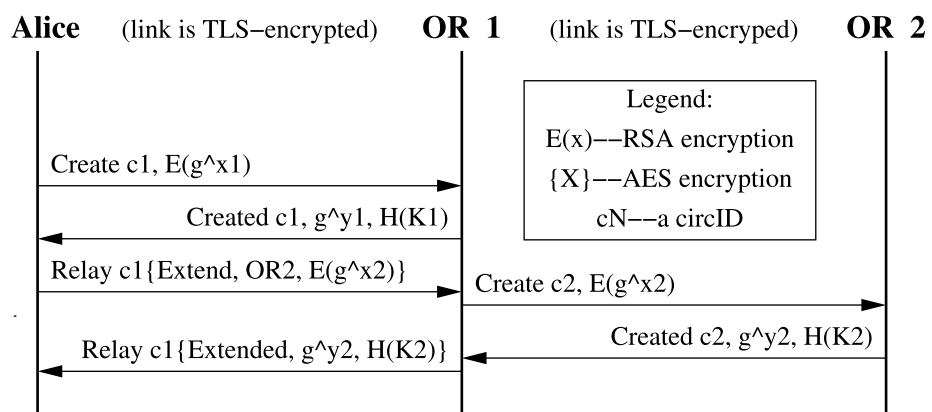
\includegraphics[width=\columnwidth]{img/circuit_creation.png}
	\caption{Creating a circuit with two onion routers. Taken from \cite{tor2004original} and slightly edited.}
	\label{img_circuit_creation}
\end{figure}

When Alice wants to extend this circuit to the next onion router Carol she sends a relay extend cell to Bob, which contains the address of Carol as well as a DH parameter \(g^{x_2}\) encrypted with Carols onion key. This data is encrypted symmetrically with AES-128 and the already negotiated key \(K\) between Alice and Bob.\\
Bob decrypts this information, chooses a unused circuit identifier between Carol and him and forwards the information received from Alice to Carol in a new \textit{create} cell. The same process as already described takes place on Carols side and she sends \(g^{y_2}\) back to Bob after computing the key \(K_2 = g^{x_2y_2}\). Bob encrypts this information with \(K\) and sends it back to Alice who can also compute \(K_2\) then. The circuit is extended by another onion router now and Alice has a key shared with Bob and one shared with Carol.

\subsection{Sending TCP data through a circuit}

After having established a circuit Alice can start to send data over the Tor network. This is illustrated below for the simple case of requesting a website.

\begin{figure}
	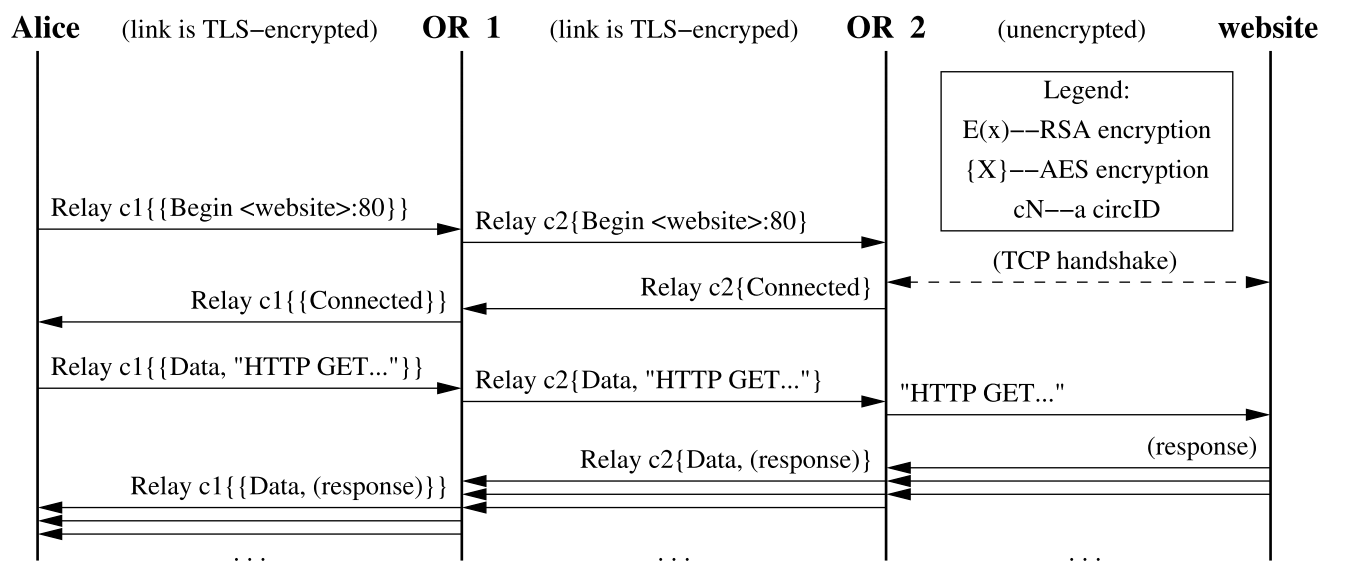
\includegraphics[width=\columnwidth]{img/http_request.png}
	\caption{Requesting the content if a website via HTTP over an established circuit. Taken from \cite{tor2004original} and slightly edited.}
	\label{img_http_request}
\end{figure}

\section{Improvements to onion routing}

%goals
In case of Tor the usability is a security requirement because it hide users among users and a system with fewer users provides less anonymity.


Additionally to onion routing, Tor added perfect forward secrecy, congestion control, directory servers, integrity checking, configurable exit policies and a practical design for location-hidden services via rendezvous points.

\textbf{Perfect forward secrecy:} In the original onion routing design a single hostile node can record traffic and later compromise succesive nodes in the circuit. To avoid this Tor uses an incremental path building design. Thant means, that the initiator negotiates session keys with each succecive node in the circuit. If these keys are deleted, the compromised nodes are not able to decrypt old traffic.

\textbf{Congestion control:} If many users choose the same OR-to-OR connectionin their circuits, that connection can be saturated. Without any congestion control this bottleneck can propagate through the whole network. To avoid this, Tor is able to control the circuits bandwidth in each OR. 

\textbf{Directory servers:} Both Onion routing and Tor has to send periodically state informations (known ORs with their current states) to their users. In the onion routing design they flood their network with these state informations. Tor uses so called \textit{directory servers} to distribute this informations through the network. The users download them periodically every 15 minutes via HTTP.

\textbf{Integrity checking:} Tor uses TLS between its nodes. Because of that an adversary is not able to change the content of the data.

\textbf{Rendezvous points:} If a user wants to connect with a hidden server the onion routing design uses long lived "reply onions", which are used to build a circuit to a hidden server. This is bad because the onion routing design does not provide forward security. For a connection between an user and a hidden server, tor uses so called rendezvouz points. If a user wants to create a connection to a hidden server, it uses the introduction points of this hidden server to send them a rendezvous point. The user and the hidden server uses this rendezvous point to create a circuit between them. Every hidden server has circuits to ORs, which are introduction points.\cite{rendezvousPoints}